
\section{Evaluation}
\label{sec:eval}

\christos{todo list: a) study of adaptive batching (fixed with various
  sizes vs adaptive), b) some breakdown of processing before/after to
  show how things change with IX, c) fix FIN/RST issue in our
  microbenchmark}

We compared \ix to a baseline running the most recent Linux kernel and to
mTCP~\cite{jeong2014mtcp}. Our evaluation uses both networking
microbenchmarks and a real-world, massively deployed, event-based
application. In all cases, we consider TCP.

\subsection{Experimental Methodology}
\label{sec:eval:setup}


%We use two experimental setups because we wish to simultaneously
%compare with mTCP and scale to bandwidth beyond 10GbE.  Unfortunately,
%our 4x10GbE setup uses recent hardware not supported by mTCP out of
%the box\footnote{We were able to port mTCP to the 4x10GbE setup, but
%  could not reach the expected performance.  We will attempt to unify
%  the setup by the camera-ready deadline.}.  Linux and \ix run on both
%setups.

\begin{figure}
\begin{centering}

\includegraphics{figs/pingpong.eps}
\caption{NetPIPE performance for varying message sizes and system software configurations.}
\label{fig:pingpong}
\end{centering}
\end{figure}

 

%Stanford cluster
%\myparagraph{10GbE setup:} This setup
%consists of a cluster of 28 Xeon E5-2630 @ 2.3 Ghz machines with Intel
%82599EB 10GbE and Solarflare SFC9000 10GbE NICs, configured with 64 GB
%of RAM each. They are connected with an Arista 7050S-64 switch. One
%machine with an Intel NIC is used as the server, while the rest are
%used as clients. The server socket has 6 cores and 12 hyperthreads.


%% put the key last to have correct numbering

\begin{figure}

\centering
 \subfloat[10GbE: Multi-core scalability (n=1;s=64B)]{
  \label{fig:short10:mcore}
   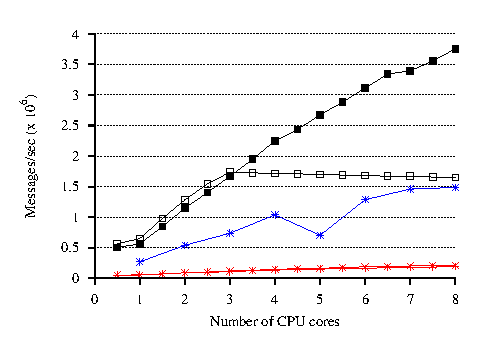
\includegraphics{figs/short-mcore-v2.eps}}
 \hspace{.01in}
 \subfloat[10GbE: $n$ roundtrips per conn. (s=64B)]{
  \label{fig:short10:roundtrips}
  
\includegraphics{figs/short-roundtrips-v2.eps}}
  \hspace{.01in}
 \subfloat[10xGbE: Different message sizes $s$ (n=1)]{
  \label{fig:short10:size}
  
\includegraphics{figs/short-size-v2.eps}}
 \centering

  \vspace{-7.8in}
  \subfloat{
\includegraphics{figs/short-key-v2.eps}}
 \vspace{7in}



\caption{Short message performance on the 10GbE and 4x10GbE setups.}
 \label{fig:shortboth}

\end{figure}



Our experimental setup consists of a cluster of 18 clients
and one server connected by
a Quanta/Cumulus 48x10GbE switch with a Broadcom Trident+ ASIC.
The client machines are a mix of Xeon E5-2637 @ 3.5 Ghz and Xeon
E5-2650 @ 2.6 Ghz. The server is a Xeon E5-2665 @ 2.4 Ghz with
256 GB of DRAM.  Each client and server
socket has 8 cores and 16 hyperthreads. All machines are configured
with Intel x520 10GbE NICs (82599EB chipset). We connect clients
to the switch through a single NIC port, while for the server it depends
on the experiement. For \emph{10GbE} experiments we use a single
NIC port, and for \emph{4x10GbE} experiments we use four NIC ports
bonded by the switch with a L3+L4 hash.

Our baseline configuration in each
machine is an Ubuntu LTS 14.0.4 distribution, updated to the 3.16.1 Linux kernel, the most
recent at time of writing.
%When reporting multi-core scalability, we report
%results on a per-core basis.
We enable hyperthreading when it improves performance. Except for
\S\ref{sec:eval:netpipe}, client machines always run Linux. All power
management features are disabled for all systems in all
experiments. Jumbo frames are never enabled.


The Linux client and server implementations of our benchmarks use the
\texttt{libevent} framework with the \texttt{epoll} system call.  We
downloaded and installed mTCP from the public-domain
release~\cite{url:mtcp}, but had to write the benchmarks ourselves
using the mTCP API.  To run mTCP, we switch to the 2.6.36 kernel, as
this is the most recent supported kernel version.  We report only
10GbE results for mTCP, as it does not support NIC bonding.


\subsection{Latency and Single-flow Bandwidth}
\label{sec:eval:netpipe}

We first evaluated the latency of \ix using NetPIPE, a popular
ping-pong benchmark, using our 10GbE setup.  NetPIPE simply exchanges
a fixed-size message between two servers and helps calibrate the
latency and bandwidth of a single flow~\cite{snell1996netpipe}.  In
all cases, we run the same system (Linux, mTCP, or \ix) on both ends.

\edb{NEW:}Fig.~\ref{fig:pingpong} shows the goodput achieved for different
message sizes.  Two \ix servers have a one-way latency of
5.7\microsecond (using 64B messages) and achieve goodput of 5Gbps
(half of the maximum) with messages as small as 20KB. In contrast, two
Linux servers have a one-way latency of 24\microsecond and require
385KB messages to achieve 5Gpbs.  The differences in system
architecture explain the difference: \ix has a dataplane model that
polls queues and processes packets to completion whereas Linux has an
interrupt model, which wakes up the blocked process.  
As for mTCP, its use of aggressive batching to offset the cost of
context switching~\cite{jeong2014mtcp} comes at the expense of low
latency, and it underperforms \ix and Linux in this particular test.




\subsection{Scalability and High Connection Churn}
\label{sec:eval:short}



Next, we evaluate \ix's multi-core scalability and ability to handle workloads
with extreme connection churn by using the same benchmark used to
evaluate MegaPipe~\cite{DBLP:conf/osdi/HanMCR12} and
mTCP~\cite{jeong2014mtcp}. Multiple clients connect to a single server
listening on a single port, send a request of size $s$, and wait for an
echo of a message of the same size.  As with NetPIPE, while receiving
the message, the server holds off its echo response until the message
has been entirely received.  Each client performs this synchronous
remote procedure call $n$ times before closing the connection.
As in ~\cite{jeong2014mtcp}, clients close the connection using a
reset (\texttt{TCP RST}) to avoid exhausting ephemeral ports.
\dm{This begs the question of what happens
  with FIN, since that is more realistic\@.  Is the point that \ix has
an unfair advantage?} \adam{(1) how do we get linux clients to send
TCP RST? (2) Does the fact that IX will only close with TCP RST matter
and why is this?}


%%
%% RAW DATA - 1024 message per connection
%% IX:  7074246
%% mTCP: 3253521

Figs.~\ref{fig:short10:mcore}-\ref{fig:short10:size} show the results
for both the 10GbE and the 40GbE configurations.  For the 10GbE
configuration, the results for Linux and mTCP are consistent with those
published in the mTCP paper~\cite{jeong2014mtcp}.  For all three
tests (core scaling, message count scaling, message size scaling), \ix
scales more aggressively than mTCP and
Linux. Fig.~\ref{fig:short10:mcore} shows that \ix needs only 3 cores
to saturate the 10GbE link whereas mTCP requires all 8 cores. On
Fig.~\ref{fig:short10:roundtrips} for 1024 rountrips, \ix delivers \george{CHECK}8.8
million messages per second, which is 1.9x the throughput of mTCP and
of and \george{CHECK} 8.8x that of Linux. For this packet rate we
have achieved line rate and are limited only by 10GbE bandwidth.

%% PROOF of line rate:
% 10 * 10 ^ 9 bits  / (12 interframe gap + 7 preamble + 1 start frame delimiter +
%		       14 ethernet hdr + 20 IP hdr + 20 TCP hdr + 64 payload + 4 CRC) bytes
% = 8 802 816.9 requests / second

Figs.~\ref{fig:short10:mcore}-\ref{fig:short10:size} shows that
\ix can scale beyond 10GbE to a 4x10GbE configuration.
Fig.~\ref{fig:short10:mcore} shows that \ix linearly scales to deliver
\data{3.9}{3.8}million TCP connections per second on 4x10GbE.
Fig.~\ref{fig:short10:roundtrips} shows a speedup of 128\% with $n=1$
and of 30\% with $n=1K$ over the 10GbE configuration.  Finally,
Fig.~\ref{fig:short10:size} shows \ix can deliver 8KB messages with a
goodput of \data{35}{34.5}Gbps, for a wire throughput of \data{38}{37.9}Gpbs (out of
a possible 39.7Gbps).  Overall, \ix makes it practical to scale
protected TCP/IP processing beyond 10GbE, even with a single socket
multi-core server.

\subsection{Connection Scalability}

\label{sec:eval:scale}

We also evaluate \ix's scalability when handling a large number of
concurrent connections on the 4x10GbE setup. In this benchmark, the 18 client machine each run
$n$ threads, with each thread repeatetly performing a 64B remote
procedure call to the server with a variable number of open connections. \adam{Should
we emphasize that all connections are active not just open?}
We experimentally set $n=24$ to maximize throughput.  We report
the maximal throughput in messages per second for a range of
total established connections.

%Connection scaling IX/Linux @ 40Gbe 
%12036405.031689
%915256.419191
%/p
%13.15085


Fig.~\ref{fig:connscaling} shows up to to \data{100,000}{250,000} connections, which
is the upper bound we can reach with the available client machines.
As expected, throughput increases with the degree of concurrency, but
then decreases for very large connections counts due to the
increasingly high cost of multiplexing among open connections.  At the
peak, \ix performs \data{13x}{10x} better than Linux, consistent with the results
from Fig.~\ref{fig:short10:roundtrips}.  

With 250,000 connections and
4x10GbE, \ix is able to deliver  \data{53}{47}\% of its own peak throughput.
We verified that the drop in throughput is not due to an increase in
instruction count, but instead can be attributed to the performance of
the memory subsystem. Indeed, Intel's Data Direct I/O technology, an
evolution of DCA~\cite{DBLP:conf/isca/HuggahalliIT05}, eliminates nearly all
cache misses associated with DMA when given enough time between polling intervals,
resulting in as little as 1.4 L3
cache misses per message for up to 10,000 concurrent connections.  In
contrast, the workload averages 25 L3 cache misses per message when
handling 250,000 concurrent connections.  Clearly, the working set of
this workload, which is dominated by the TCP connection state, cannot
fit into the processor's L3 cache.  Nevertheless, we believe that
further optimizations in the size and access pattern of lwIP's TCP/IP
protocol control block structures could substantially reduce the
impact of the memory subsystem.
  



\subsection{Memcached Performance}
\label{sec:eval:memcached}



%FIXME if different keys


\begin{figure*}[t]

\centering
  \vspace*{0.3in}
 \subfloat[Throughput for varying established connections]{
  \label{fig:connscaling:throughput}
   
\includegraphics[width=.49\textwidth,clip]{figs/blank.eps}}
 \hspace{.02in}
 \subfloat[Avg. and 99\% latency for varying established connections]{
  \label{fig:connscaling:lat}
  
\includegraphics[width=.49\textwidth,clip]{figs/blank.eps}}
\centering
  \vspace{-2.8in}
  \subfloat{
\includegraphics[width=1\textwidth,clip]{figs/short-key.eps}}
 \vspace{2.3in}
 \
\caption{Connection scaling}
 \label{fig:connscaling}

\end{figure*}

\begin{figure*}
\begin{centering}
\subfloat[Latency vs throughput for the memcached ETC workload.]{

\includegraphics{figs/memcached-etc-basic.eps}}
\subfloat[Multilate-Me Again!]{

\includegraphics{figs/blank.eps}}
\caption{Capacity and quality of service of memcached on Linux and \ix for XXX and YYY concurrent, established connections}
\label{fig:mutilate}
\end{centering}
\end{figure*}



Finally, we evaluated the performance benefits of the \ix protected
dataplane design with \texttt{memcached}, a massively deployed,
in-memory key-value store built on top of the \texttt{libevent}
framework~\cite{url:memcached}. It is frequently used as a
high-throughput, low-latency caching tier in front of persistent
database servers. \texttt{memcached} is a network-bound
application, with threads spending over 80\% of execution time in
kernel mode for network processing~\cite{Leverich:RHSU:2014}. It is a
difficult application to scale, in particular because the
common deployments involve high connection counts for
\texttt{memcached} servers and small-sized requests and
replies~\cite{nishtala2013scaling,Atikoglu:2012:WAL}

We use the \texttt{mutilate} load-generator to place a selected load
on the server in terms of requests per second (RPS) and measure
response latency~\cite{url:mutilate}. \texttt{mutilate} coordinates a
large number of client threads across multiple machines to generate
the desired RPS load, while a separate unloaded client measures
latency by issuing one request at the time.  We configure
\texttt{mutilate} to generate load representative of two workloads
from Facebook~\cite{Atikoglu:2012:WAL}: the ETC workload that
represents that highest capacity deployment in Facebook, has 20B - 70B
keys, 1B-1KB values, and 90\% GET requests; and the USR workload that
represents deployment with most GET requests in Facebook, has short
keys ($<$20B), 2B values, and 99\% GET requests. In USR, almost all
traffic involves minimum-sized TCP packets. Each request is issued 
\dm{incomplete sentence?}

\dm{Paragraph needs editing.  Also, why not report 99\% or 99.9\%?}
\adam{Are our linux graphs too noisy to do 99th? IX looks fine at 99th...}
For all experiments, we report 95th percentile latency as a function
of the achieved throughput as this is the relevant metric for
datacenter
applications\microsecond~\cite{DBLP:journals/cacm/DeanB13}. This graph
provides insights the full range of system behaviors. Most commercial
\texttt{memcached} use such a latency-throughput graph to provision
each server so that the 95th percentile latency does not exceed 200 to
500.  We carefully tune the Linux baseline setup according to the
guidelines in \cite{Leverich:RHSU:2014}. Specifically, we pin
memcached threads, configure interrupt-distribution based on
thread-affinity, and tune interrupt moderation thresholds. We believe
that our baseline Linux numbers are as tuned as possible for this
hardware using the open-source version of
\texttt{memcached-1.4.18}. For our benchmark, we use 6 client machines
and a total of 772 connections to the memcached server. We report the
results for the configuration that provides the best performance: 
8 sockets with Linux, but only 6 with \ix.

\christos{Should we discuss the porting process to IX?}
\adam{new:} Porting memcached to IX primarly consisted of adapting it
to use our event library. In most cases, the port was straightforward,
replacing Linux and \texttt{libevent} function calls with their equivalent
versions in our API. There were a few incompatibilities that required
aditional effort. For example we don't yet support vectored write
operations (e.g., \texttt{writev}) in our
API (the benefits would be only marginal because we batch
writes inside our event library). Morever, we had to make some internal changes
to memcached in order to deliniate the spawning elastic threads and background
threads.  \adam{On our haswell machine, which runs an older linux
kernel this change works great, but it had to be disabled on the mavericks and at EPFL because
newer kernels have something wierd going on with thread spawning. In pratice,
background threads didn't make any noticable difference on the Haswell. Should I say anything about this
limitation?} Finally, we made some small changes to the behavior of the main
event loop in order to better support our run to completion execution model. We
did not attempt to tune the internal scalability of memcached or adapt memcached
to support zero-copy IO operations.


%%
%% see  figs/data/memcache-sla-qps.txt

%82.5  139.6  650K
%42.0  54.3   1320K  --> 2.03x     --> 2.0x
%79.6  136.8  580K
%37.7  44.5   1620K  -->  2.74519  --> 2.7x


\begin{table}[b]
%\vspace{-1em}
\begin{center}
\begin{small}
\begin{tabular}{|l|c|c|c|}
\hline
%Configuration &  \multicolumn{2}{|c|}{Unloaded latency} &  QPS for SLA:\\
Configuration &  Minimum latency &  RPS for SLA:\\
&  @99th pct &  $<500$\microsecond@99th pct\\
\hline
ETC-Linux & 93\microsecond & 500K\\
ETC-IX    & 46\microsecond & 1500K\\
\hline
USR-Linux & 84\microsecond & 450K\\
USR-IX    & 31\microsecond & 2150K\\

\hline
\end{tabular}
\caption{Unloaded latency and maximum RPS for a given service-level agreement for the memcache workloads \texttt{ETC} and \texttt{USR}.}
%\vspace*{-2em}
\label{tbl:mutilate}
\end{small}
\end{center}
\end{table}



\edb{NEW with table:} Fig.~\ref{fig:mutilate} shows the throughput-latency curves for the
two \texttt{memcached} workloads for Linux and \ix, while
Table~\ref{tbl:mutilate} reports the unloaded latencies and maximum query throughput that meets a service-level agreement of $<1ms$ at the 95th percentile.
\ix noticeably reduces the unloaded latencies, also measured
at the 95th percentile.  We note here that the benchmark
clients are running on Linux, and that running them on \ix should
further reduce that latency. 

\edb{NEW:}For both workloads, the distribution of CPU time shifts from being
$>80\%$ in the kernel with Linux to $<30\%$ with \ix.  Since the
application is unmodified, Amdahl's law would predict a speedup of 3x.
\ix actually increases the throughput of memcached by 1.8 and 2.7
for \texttt{ETC} and \texttt{USR}, respectively.  We explain the
difference by the increased lock contention within the application
itself, in particular for \texttt{ETC}, which has a higher write frequency.


%
\subsection{Multi-tier Performance}

\edb{THIS IS A STRECH STRETCH GOAL} 

Evaluating the performance of a highly-scalable, multi-tier
environment in a lab environment is challenging on multiple fronts:
first, there are ---to the best of our knowledge--- no universally
accepted multi-tier benchmarks that involve key-value stores and in
general that are representative of web-scale applications.  Second,
most lab enviornments are orders of magnitude smaller than a
datacenter.

Therefore, we construct a simple, synthetic multi-tier benchmark that
mimics the behavior of a social application stored in an in-memory
key-value store.  The application is a simple \texttt{http} server
that returns the top-most recent update among a users list of friends.
The application server parses the http request to
get the userid, uses the user id to return a friends-list from a
key-value store, and then queries the key-value store individually for
each friend for the most recent value.  It then processes replies and
return the top-most entries.  In our experiments, we model a database
with $10^7$ million users, each with 100 friends. 

We scale the benchmark to model a cluster deployment with $\alpha$
client connections per application server, $\beta$ httpd and $\gamma$
memcached servers.  Keys are distributed uniformly between the
$\gamma$ servers.  We model a large-scale deployment with
$\alpha=10^5$, $\beta=10^4$ and $\gamma=10^4$ on a deployment that consists of 4
actual application servers and 1 memcached server (running on our
server hardware with 4x10GbE connectivity).  Each application server
runs \texttt{lighthttpd} with the application logic written directly
within the server, and maintains a distinct connection for each of the
$\alpha$ virtual clients and $\gamma$ virtual nodes.  The key-value store is
running \texttt{memcache} as described in \S\ref{sec:eval:memcache}.
We use the remaining 14 client machines to simulate $4 \times \alpha$
clients and the 19th client to measure the latency of the application.

Fig.~\ref{missing} reports the latency as a function of the
throughput, as determined by varying the client load.  We compare a
Linux baseline with one in which \ix is used to run both the
application server and the memcached server.  We note that the choice
of operating system on the application server determines the number of
concurrent connections. Indeed, because of the coherence-free
execution model, each application server needs to open a distinct TCP
flow to the same virtual node for each of its hardware threads.

\edb{OPTIMISTIC: } Fig.~\ref{missing} shows that \ix can saturate the
hardware connectivity.  Indeed, the bottlneck consits of the
communication 







